В этой главе мы рассмотрим какие результаты 
получились в ходе решения системы 
\begin{equation}
\begin{split}
    & N = - \min (\Tr(W \rho)) \\
    & \text{s.t.} \Tr(W) = 1 \\
    & \forall M: W = P_M + Q_M^{T_M}, Q_M \geq 0, P_M \geq 0
\end{split}
\end{equation}
методом полуопределенного программирования для разных состояний и их конфигураций.
Задача была решена с помощью библиотеки CVXPY \url{https://www.cvxpy.org/}. Она представляет собой интерфейс, набор функций и классов, который помогает составить и решить задачу SDP на языке python.


Рассмотрим \textbf{состояния Вернера} \cite{PhysRevA.40.4277} - семейство состояний на пространстве $\mathbb{C}^d\otimes\mathbb{C}^d$, которые инвариантные относительно унитарных преобразований $U \otimes U$, $\rho_{wer} = (U \otimes U)\rho_{wer} (U^{\dag} \otimes U^{\dag})$. Семейство можно параметризовать следующим образом
\begin{equation}\label{werner-state-def}
    \rho_{wer}(p,d) = \frac1{d^2 + pd}\left(\mathbb{1} + p\sum_{i,\,j=0}^{d-1}\,\ket{i,\,j}\bra{j,\,i}\right),
\end{equation}
где $p \in [-1, 1]$. Для случая $d=2$ матрица плотности будет иметь следующий вид
\begin{equation}\label{werner-state}
    \rho_{wer}(p, 2) = \frac{1}{2(2 + p)}
    \begin{pmatrix}
        p+1 & 0 & 0 & 0 \\
        0 & 1 & p & 0 \\
        0 & p & 1 & 0 \\
        0 & 0 & 0 & 1+p \\
    \end{pmatrix}.
\end{equation}

Посчитаем меру сцепленности для цепочки из двух состояний Вернера $\rho_{wer}(p_1,2) \otimes \rho_{wer}(p_2,2)$. В статье \cite{sun-chen-21} было доказано, что данное состояние является сцепленным при следующих параметрах $p_1$ и $p_2$

\begin{equation}\label{2-warn-states-entang-region}
    -1\,\leqslant\,p_1\,\leqslant -0.940198;\quad -1\,\leqslant\,p_2\,\leqslant\,-0.94066.
\end{equation}

Проведём аналогичные численные расчеты. Возьмем два состояния, параметризованные $p_1$ и $p_2$ соответственно, и проанализируем как будет меняться сцепленность состояния $\rho_{wer}(p_1,2) \otimes \rho_{wer}(p_2,2)$ при изменении параметров $p_1$ и $p_2$. Решение SDP задачи \ref{sdp-task-main} показано на рис. \ref{ris:sdp-2-warn-states}. Точки, в которых $N(p_1, p_2) > 0$, соответствуют состояниям, которые не являются PPT-смесью, и, следовательно, являются истинно сцепленными. По графику видно, что произведение сцепленных состояний не всегда является истинно сцепленным. Действительно, в противном случае график имел бы квадратную форму, а не треугольную. Также стоит отметить, что область сцепленности, оказалась гораздо больше, чем предполагалось ранее \ref{2-warn-states-entang-region}.

\begin{figure}[h]
    \center{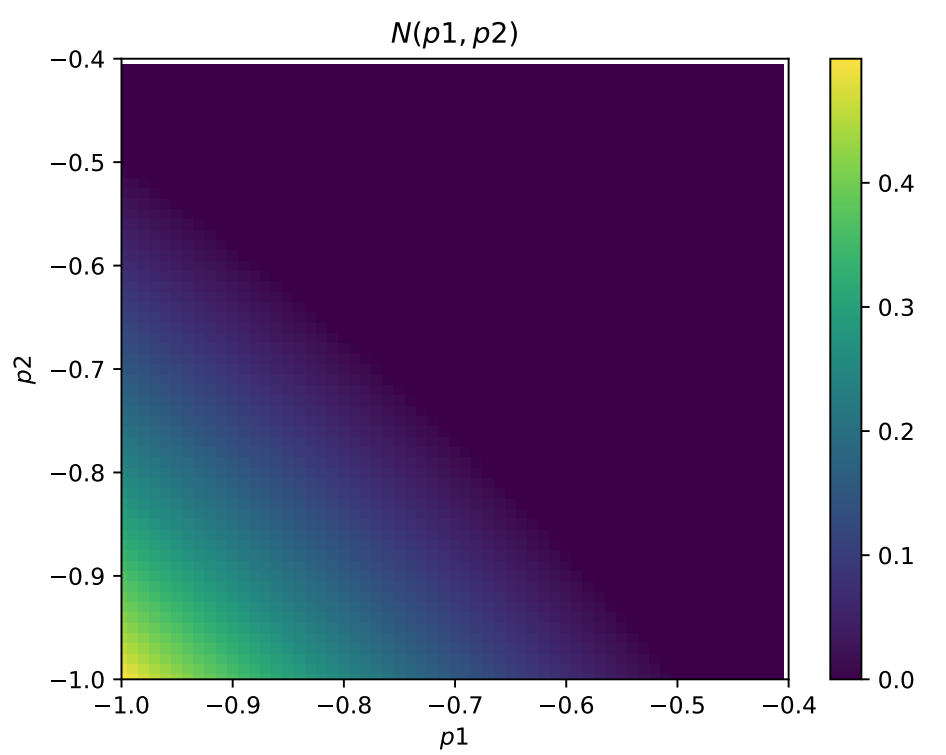
\includegraphics[width=0.7\linewidth]{img/2-werner-3d-simple.png}}
    \caption{
    Численный результат SDP задачи \ref{sdp-task-main} для 
    состояния $\rho_{wer}(p_1,2) \otimes \rho_{wer}(p_2,2)$ при разных значениях параметров $p_1$ и $p_2$. Точки, в которых $N(p_1, p_2) > 0$, соответствуют истинно сцепленным состояниям. По графику видно, что произведение сцепленных состояний не всегда является истинно сцепленным. Действительно, в противном случае график имел бы квадратную форму, а не треугольную.
    }
    \label{ris:sdp-2-warn-states}
\end{figure}

Проведем аналогичные вычисления с изотропным состоянием. \textbf{Изотропные состояния} - это семейство состояний, определенных на пространстве $\mathbb{C}^{d} \otimes \mathbb{C}^{d}$, которые инвариантны относительно унитарных преобразований следующего вида $U \otimes U^{*}$. Их можно параметризовать следующим образом
\begin{equation}\label{isotropic-state}
    \rho_{iso}(p, d) = p \ket{\phi^{+}_d}\bra{\phi^{+}_d} + \frac{1-p}{d^2}\mathbb{1},
\end{equation}
где $\ket{\phi^{+}_d}$ - $d$-мерное максимально сцепленное состояние $\ket{\phi^{+}_d} = \frac{1}{\sqrt{d}}\sum\limits_{i=0}^{d-1}\ket{ii}$.

При $d=2$ матрица плотности изотропного состояния будет иметь следующий вид
\begin{equation}\label{isotropic-state-2dmatrix}
    \rho_{iso}(p, 2) = \frac{1}{4}
    \begin{pmatrix}
        p+1 & 0 & 0 & 2p \\
        0 & p-1 & 0 & 0 \\
        0 & 0 & p-1 & 0 \\
        2p & 0 & 0 & p+1 \\
    \end{pmatrix}.
\end{equation}
Рассмотрим, как и в прошлый раз, цепочку из двух изотропных состояний $\rho_{iso}(p_1,2) \otimes \rho_{iso}(p_2,2)$ и построим аналогичный график. Результат представлен на рис. \ref{img:2-isotropic}а.

В статье \cite{Contreras_Tejada_2022} приводился аналитический анализ сцепленности изотропных состояний, в частности там было доказано, что цепочка из двух одинаковых изотропных состояний будет истинно сцепленной, если параметр $p$ будет удовлетворять следующему неравенству
\begin{equation}\label{isotropic-bisep-analitic-bound}
    p > \frac{(1 + \sqrt{2})d - 1}{d^2 + 2d - 1}.
\end{equation}
Для случая $d=2$ неравенство примет вид $p > 0.5469$. На рис. \ref{img:2-isotropic}a нарисована прямя $p_2 = p_1$, на которой изображена нижняя теоретическая граница. После нее состояние является истинно сцепленным. На срезе графика по прямой $p_2 = p_1$, представленным на рис. \ref{img:2-isotropic}b видно, что теоретическая граница и экспериментальная согласуются в пределах погрешности.

\begin{figure}
    \subfigure[]{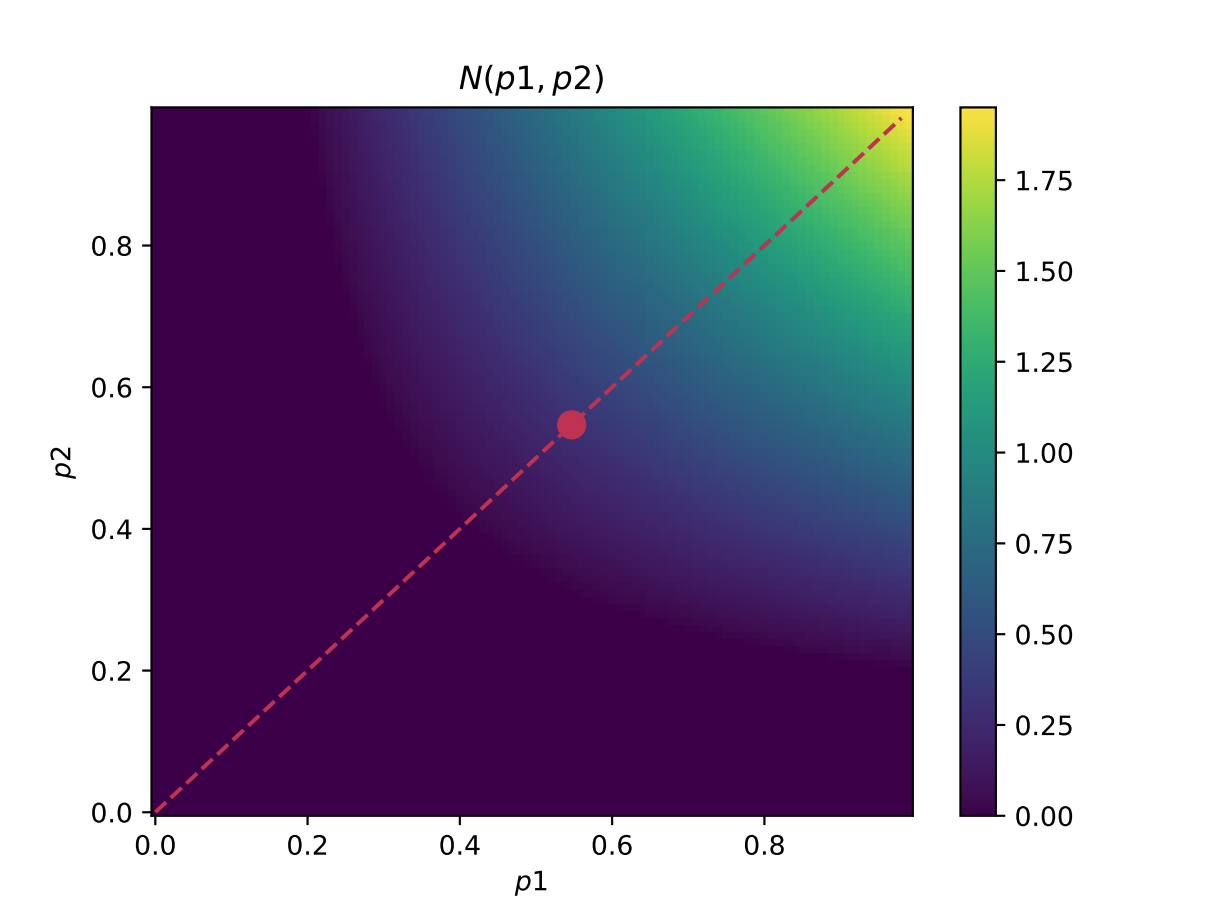
\includegraphics[width=0.55\textwidth]{img/2-isotropic-3d.png}}
    \subfigure[]{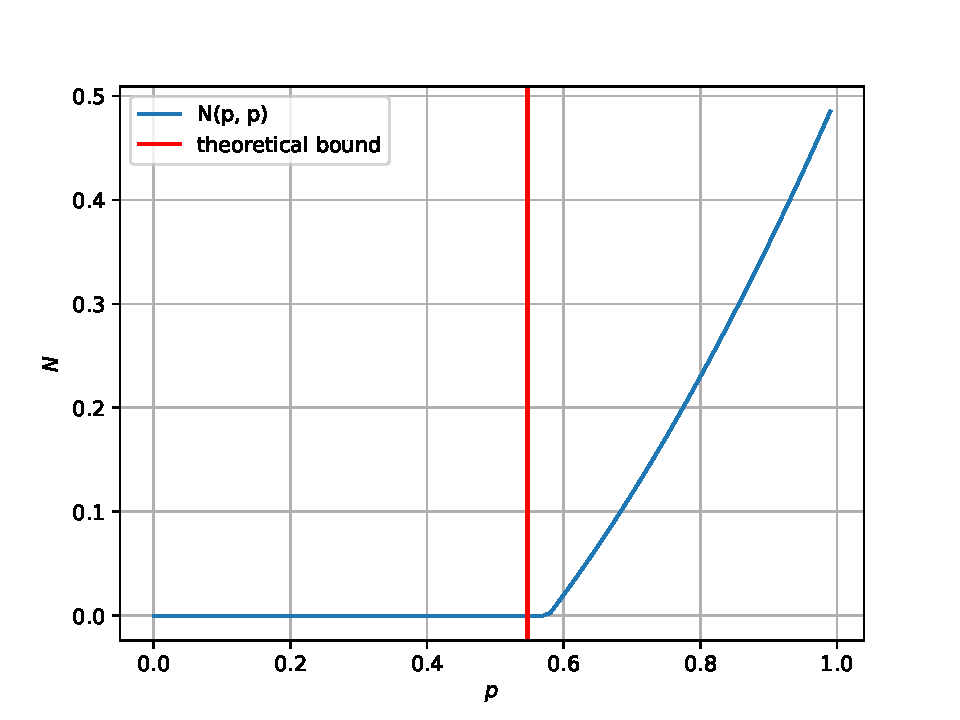
\includegraphics[width=0.55\textwidth]{img/2-isotropic-2d.pdf}}
    \subfigure[]{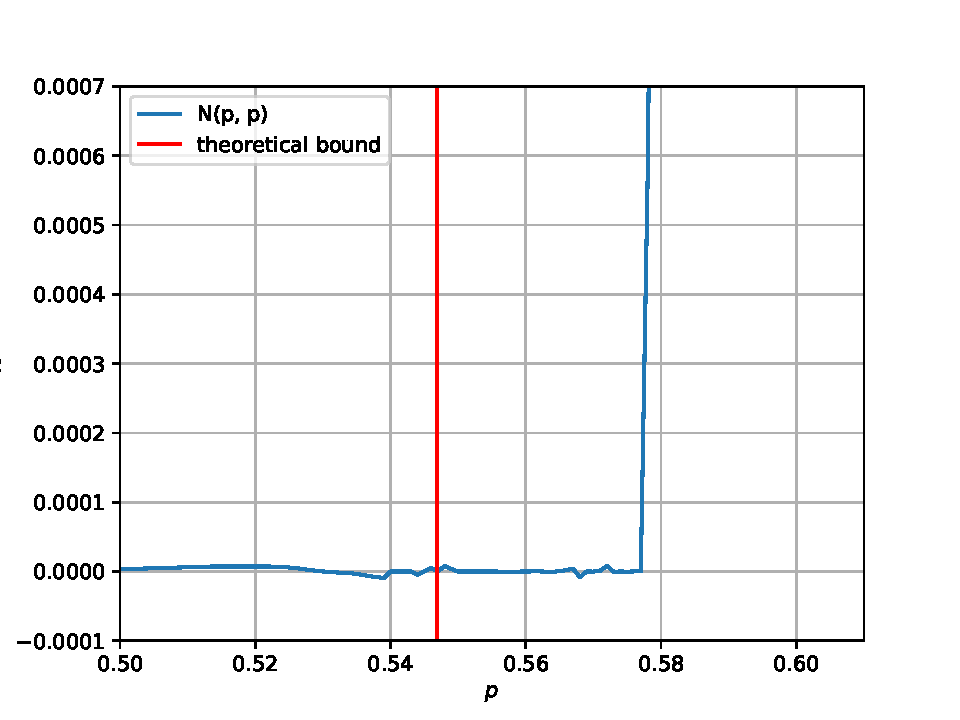
\includegraphics[width=0.55\textwidth]{img/2-isotropic-2d-detail.pdf}}
    \caption{
    \textbf{a} - численный результат SDP задачи \ref{sdp-task-main} для состояния $\rho_{iso}(p_1,2) \otimes \rho_{iso}(p_2,2)$ при разных значениях параметров $p_1$ и $p_2$. Точки, в которых $N(p_1, p_2) > 0$, соответствуют истинно сцепленным состояниям. Красная прямая $p_2 = p_1$ и точка на ней, показывает нижнюю теоретическую границу, после которой состояние является сцепленным.
    \textbf{b} - представлен срез графика a по прямой $p_2 = p_1$.
    \textbf{c} - представлен более детальный график b в точке излома.}
    \label{img:2-isotropic}
\end{figure}

Заметим, что аналитическую границу сцепленности \ref{isotropic-bisep-analitic-bound} можно применить и к семейству состояний Вернера.
Действительно, матрицу плотности для $d=2$ состояния Вернера можно представить в следующем виде
\begin{equation}
\begin{split}
    \rho_{wer}(p, 2) & = 
    \frac{1}{2(2 + p)}
    \begin{pmatrix}
        p+1 & 0 & 0 & 0 \\
        0 & 1 & p & 0 \\
        0 & p & 1 & 0 \\
        0 & 0 & 0 & p+1 \\
    \end{pmatrix}
     = \\
    &= \frac{\lambda}{4} \mathbb{1} + (1-\lambda)\ket{\psi^{-}_2} \bra{\psi^{-}_2}
     =
    \begin{pmatrix}
        \frac{\lambda}{4} & 0 & 0 & 0 \\
        0 & \frac{1-\lambda}{2} + \frac{\lambda}{4} & -\frac{1-\lambda}{2} & 0 \\
        0 & -\frac{1-\lambda}{2} & \frac{1-\lambda}{2} + \frac{\lambda}{4} & 0 \\
        0 & 0 & 0 & \frac{\lambda}{4} \\
    \end{pmatrix}, \\
\end{split}
\end{equation}

где $\ket{\psi^{-}_2}$ максимально смешенное состояние, $\ket{\psi^{-}_2} = \frac{1}{\sqrt{2}} \left( \ket{01} - \ket{10} \right)$ и $\lambda = \frac{2(p+1)}{2 + p}$.
С помощью унитарного преобразования $U$, которое не повлияет на сцепленности, можно перевести $\ket{\psi^{-}_2}$ в $\ket{\psi^{+}_2}$.
Тогда состояние Вернера, выраженное через максимально смешенное состояние, с точностью до коэффициентов, совпадет с 
 определением изотропного состояния \ref{isotropic-state}.
 Тогда теоретическую оценку границу сцепленности для изотропных состояний \ref{isotropic-bisep-analitic-bound} 
 можно примести и для состояния Вернера в случае, когда $d=2$
 \begin{equation}\label{werner-sep-2d-analytic-bound}
 \begin{split}
     & p < -\frac{2\beta(2)}{1 + \beta(2)} \approx -0.70709, \\
     & \beta(d) = \frac{(1 + \sqrt{2})d - 1}{d^2 + 2d - 1}.
 \end{split}
 \end{equation}

Сравнение полученного результата решения  SDP задачи с теоретической границей представлено на рис. \ref{img:2-werner-compare}.
\begin{figure}
    \subfigure[]{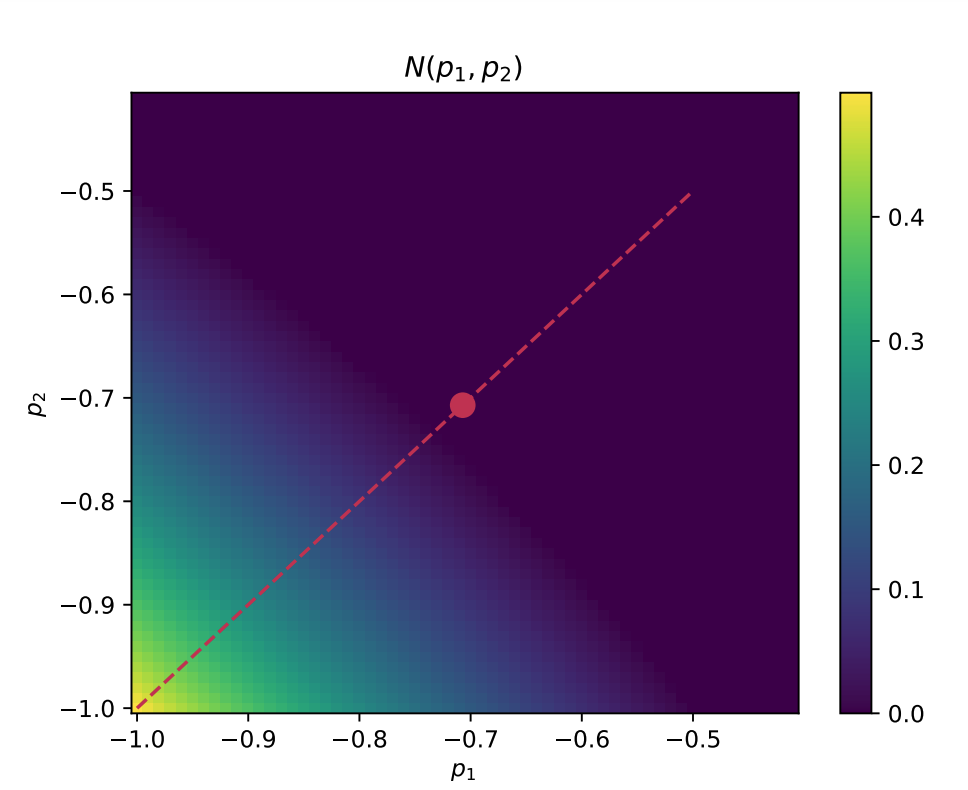
\includegraphics[width=0.55\textwidth]{img/2-werner-3d.png}}
    \subfigure[]{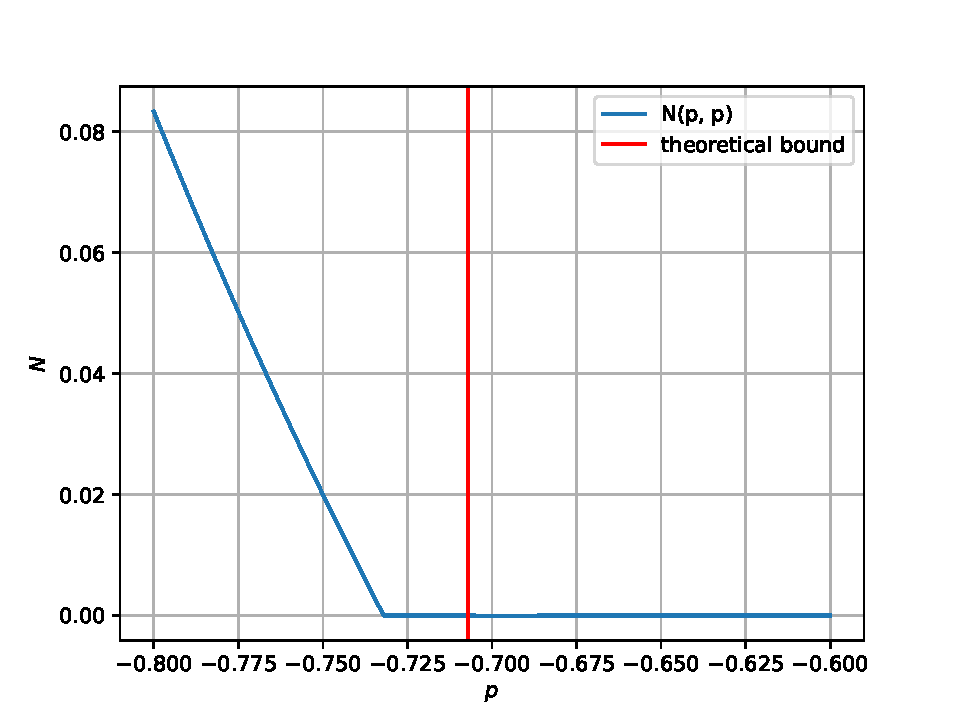
\includegraphics[width=0.55\textwidth]{img/2-werner-2d.pdf}}
    \subfigure[]{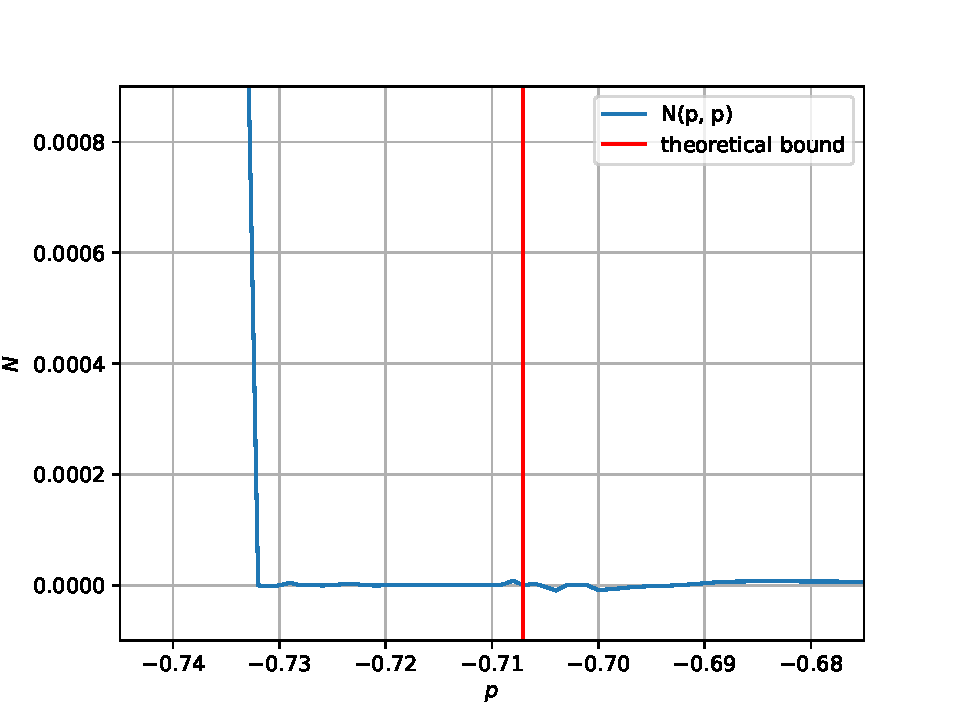
\includegraphics[width=0.55\textwidth]{img/2-werner-2d-detail.pdf}}
    \caption{
    \textbf{a} - численный результат SDP задачи \ref{sdp-task-main} для состояния $\rho_{wer}(p_1,2) \otimes \rho_{wer}(p_2,2)$ при разных значениях параметров $p_1$ и $p_2$. Точки, в которых $N(p_1, p_2) > 0$, соответствуют истинно сцепленным состояниям. Красная прямая $p_2 = p_1$ и точка на ней, показывает нижнюю теоретическую границу, после которой состояние является сцепленным.
    \textbf{b} - представлен срез графика \textbf{a} по прямой $p_2 = p_1$.
    \textbf{c} - представлен более детальный график \textbf{b} в точке излома.}
    \label{img:2-werner-compare}
\end{figure}